\documentclass[a4paper]{article}

\usepackage{geometry}
\geometry{left=1.5cm, right=1.5cm, top=2.54cm, bottom=2.54cm}
\usepackage{graphicx, hyperref, setspace, amsmath, amssymb, titlesec, fancyhdr, multicol, parskip, indentfirst, etoolbox, caption, cite, xcolor}
\usepackage{algorithm}
\usepackage{algpseudocode}
\usepackage{cuted}

\titleformat{\section}{\centering\large\scshape}{\thesection}{1em}{}
\titleformat{\subsection}{\normalsize\bfseries}{\thesubsection.}{1em}{}
\setstretch{1.0} 
\setlength{\parskip}{6pt} 
\titlespacing{\section}{0pt}{6pt}{6pt}
\titlespacing{\subsection}{0pt}{6pt}{6pt}
\titlespacing{\subsubsection}{0pt}{6pt}{6pt}

\title{Real-Time Localization Framework for Autonomous Basketball Robots}

\date{} 
\captionsetup{labelfont={small,sc}, textfont={small,sc}}

\renewcommand{\thesection}{\Roman{section}.}
\renewcommand{\thesubsection}{\textit{\Alph{subsection}.}}
\renewcommand{\thesubsubsection}{\textit{\arabic{subsubsection}.}}
\renewcommand{\thetable}{\Roman{table}} 
\renewcommand{\thefigure}{\Roman{figure}} 

\titleformat{\subsection}{\normalfont\large\itshape}{\thesubsection}{1em}{}
\titleformat{\subsubsection}{\normalfont\itshape}{\thesubsubsection}{1em}{}


\makeatletter
\renewcommand{\maketitle}{
  \begin{center}
    \noindent\rule{\textwidth}{1pt}\par
    \vspace{0.3em}
    {\LARGE \bfseries \@title \par}
    \vspace{0.3em}
    \noindent\rule{\textwidth}{1pt}\par
  \end{center}
}
\makeatother

\begin{document}

\maketitle
\vspace{1cm}


\begin{multicols}{2}
    \centering
    \textbf{Naren Medarametla}\\
    \textit{School of Computer Science Engineering}\\
    \textit{Vellore Institute of Technology}\\
    \textit{Chennai, India}\\
    \texttt{naren.medarametla2023@vitstudent.ac.in}
    \vfill\null

    \columnbreak

    \textbf{Sreejon Mondal}\\
    \textit{School of Electrical and Electronics Engineering}\\
    \textit{Vellore Institute of Technology}\\
    \textit{Chennai, India}\\
    \texttt{sreejon.mondal2023@vitstudent.ac.in}
    \vfill\null
\end{multicols}

\singlespacing
\setlength{\parskip}{6pt}
\setlength{\parindent}{0.5cm}

\begin{multicols}{2}
\setlength{\columnsep}{0.5cm}

\noindent \textbf{\textit{Abstract---}
Localization is a fundamental capability for autonomous robots, enabling them 
to operate effectively in dynamic environments. In Robocon 2025, accurate and 
reliable localization is crucial for improving shooting precision, avoiding 
collisions with other robots, and navigating the competition field efficiently. 
In this paper, we propose a hybrid localization algorithm that integrates classical 
techniques with learning-based methods, relying solely on visual data from the court’s
floor to achieve self-localization on the basketball field.
}

\small	
\noindent \textbf{
  \textit{Keywords---}\textit{Robot Localization, Autonomous Navigation, Neural Networks, Robocon}}

\section{Introduction}
\par \noindent
The DD-Robocon is the Indian national entry-level competition to Asia-Pacific Robot Contest (ABU Robocon). The objective of the competition is for college teams to design, build, and operate robots to complete certain tasks. The tasks vary each year and are usually based on cultural, historical, or technological themes related to the host country of the international contest. For Robocon 2025, the theme was Robot Basketball, where two robots had to play the game of basketball following specific rules. The arena consisted of a court of dimensions 15m $\times$ 8m and baskets at a height of 2.4m. Due to the nature of the game, the robots had to move quickly and unpredictably, and take shots from various positions on the court. The robots had to have robust and real-time self-localization determine it's distance from the basket.
In this paper we propose a vision-based localization system based on the white field lines of the basketball court.
\textbf{Section II} reviews existing methods and prior research related to this work. 
\textbf{Section III} provides a detailed description of our proposed algorithm, approach, and model architecture. 
\textbf{Section IV} provides the results obtained from our experiments. 
\textbf{Section V} evaluates the accuracy of our approach and discusses potential directions for future work.


\section{Related Work}
In our earlier methodology, we employed an odometry-based approach for the self-localization of the robots. This system integrated wheel encoders and an Inertial Measurement Unit (IMU), complemented by a TF-Luna LiDAR sensor to estimate the depth between the robot and the basket. However, the TF-Luna sensor demonstrated a limited effective range of approximately 3 to 4 meters and exhibited suboptimal accuracy within this range. Additionally, a significant challenge arose due to the absence of a clearly distinguishable object or surface on the basket, which hindered reliable depth estimation.
\par \noindent
In the subsequent approach, we employed an object detection model based on YOLOv8n, trained on a custom dataset to detect the basket. This model was utilized not only for basket detection but also for correcting the robot’s yaw orientation to ensure it consistently faced the target. To estimate the horizontal distance from the basket, we defined discrete zones, with each zone representing a specific distance range. The corresponding zone, selected manually by the pilot based on visual assessment, was then used in conjunction with the detected orientation to determine the appropriate RPM for the shooting mechanism. While this approach facilitated a simplified method for distance estimation, it was inherently dependent on manual selection and coarse approximations, which could lead to reduced accuracy and consistency.

{ \centering
  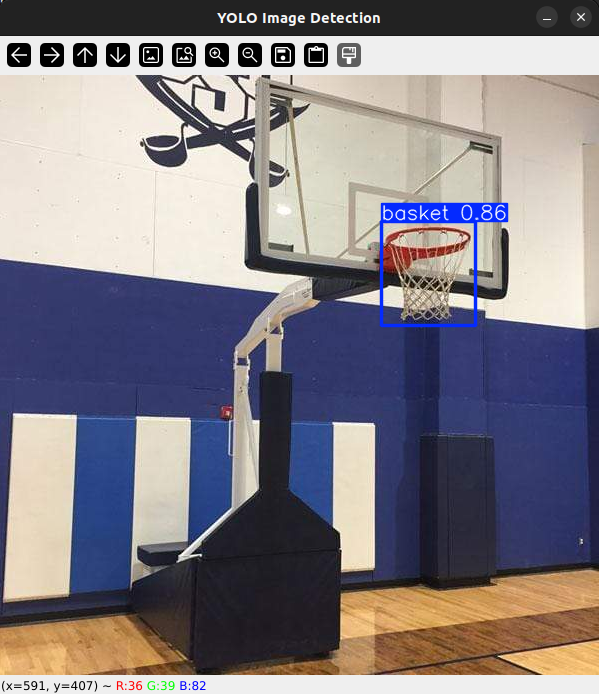
\includegraphics[scale=0.3]{results/yolo_detection.png}\\
  \captionof{figure}{basket detection}\label{fig:basket_detection}
}

\par \noindent
We improved upon the object detection approach by using the MiDaS (Multiple Depth Estimation Accuracy with Single Network) deep learning model. MiDaS is a designed for monocular depth estimation, i.e., predicting depth from a single image. It uses a ResNet-based encoder-decoder architecture, where:
\begin{itemize}
    \item The encoder extracts features from the input image.
    \item The decoder upsamples these features to produce a depth map.
\end{itemize}
The approach combines the YOLOv8 model, with the MiDaS depth estimation framework for relative depth prediction.
The pipeline begins by loading an input image, followed by inference using the YOLO model to localize the basket and identify its center. Simultaneously, MiDaS processes the same image to generate a dense relative depth map. Once the basket is detected, the relative depth at the center of the bounding box is extracted from the depth map.
An interactive calibration step is used to relate MiDaS's relative depth to real-world distance. The user is prompted to enter known ground-truth distances for three distinct positions. These pairs of relative depth and real distance are then used to fit a linear regression model, enabling real-time conversion of relative depth to metric distance.
During tracking mode, the system periodically predicts the basket's distance using the learned regression model and overlays the result on the original image alongside the visualized depth map. The output is displayed in a side-by-side format showing both RGB and color-mapped depth views for easier interpretation.

{ \centering
  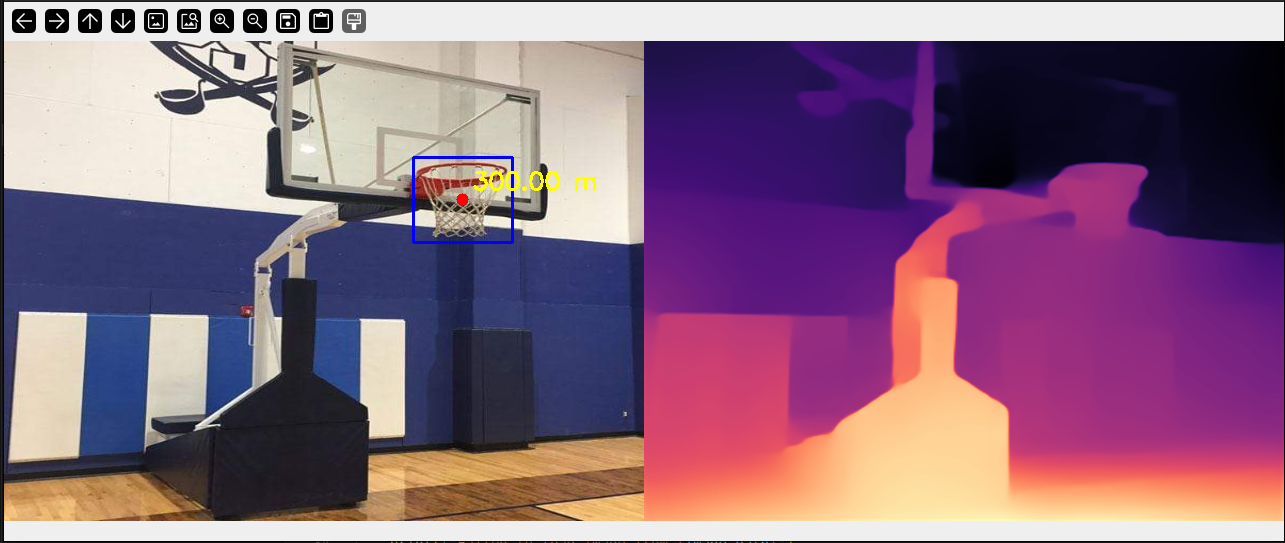
\includegraphics[width=0.4\textwidth]{results/midas.png}\\
  \captionof{figure}{basket depth estimation}\label{fig:basket_midas}
}

A key limitation of this approach was its reliance on prior calibration, which required manually measuring the distance between the robot and the basket at least three times before accurate predictions could be made. In response to these constraints, we developed the current method presented in this paper, building upon insights gained from the previous techniques.

\section{Methodology}
\par \noindent Our approach is a two-step process that begins with \textbf{Preprocessing} the image,
followed by passing it to the model for \textbf{Inference}.
\subsection{Preprocessing}
\par \noindent The input image having dimensions (640 $\times$ 480 $\times$ 3) is converted from the RGB color space to the HSV color space, then the white regions are masked out using two predefined HSV ranges.
The image is downsampled through a radial scan, flattened, and finally passed through the neural network.
Figure I shows the preprocessing pipline and Algorithm 1 gives the implementation of the downsampling algorithm.

\par \noindent

{ \centering
  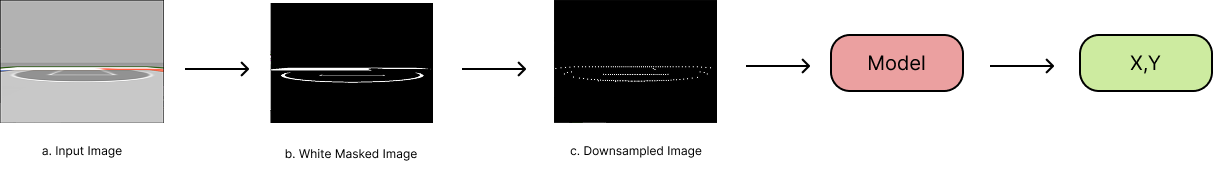
\includegraphics[width=0.5\textwidth]{results/Flowchart.png}\\
  \captionof{figure}{preprocessing pipeline}\label{fig:flowchart}
}
\begin{algorithm}[H]
  \caption{Downsampling}
\begin{algorithmic}[1]
\Statex \textbf{Input: }Image
\State $H \gets$ Image.height
\State $W \gets$ Image.width
\State $R \gets$ Black Image
\For{angle $\gets$ 0 to 180 step 2}
    \State $lastPixel \gets 0$
    \State $cx \gets \text{W / 2}$
    \State $cy \gets \text{H}$
    \For{d $\gets$ 0 to max(H, W)}
        \State $x \gets cx + d \times \cos(angle)$
        \State $y \gets cy - d \times \sin(angle)$
        \If{$0 \leq x < \text{W} \ \textbf{and} \ 0 \leq y < \text{H}$}
          \State $pixel \gets Image[y][x]$
          \If{lastPixel = 255 and pixel $\neq$ 255}
            \State $R[y][x] \gets 255 $ 
          \EndIf
          \State $lastPixel \gets pixel$
        \EndIf
    \EndFor
\EndFor
\State \textbf{Return} R
\end{algorithmic}
\end{algorithm}

\subsection{Model Architecture}
\par \noindent
The proposed model is a feedforward neural network consisting of a flattening layer followed 
by four fully connected layers. The first 200 pixels from the top of the image are removed 
to reduce the input size, as they do not carry useful information and the pixel values are scaled
down to the range [0, 1].

\par \noindent
The resulting image with dimensions (640 $\times$ 280 $\times$ 1) is flattened into a vector 
of size 1,79,200 and passed through the first linear layer, followed by a ReLU activation function.
The subsequent layers have sizes 1024, 256, and 64, each followed by a ReLU activation. 
The final layer outputs a 2-dimensional vector representing the predicted $x$ and $y$ positions of the robot.

\par \noindent
The rationale for using this relatively simple model lies in the simplicity of the input images 
and to reducing inference time.

%maybe could add input dimensions for each layer??
{ \centering
 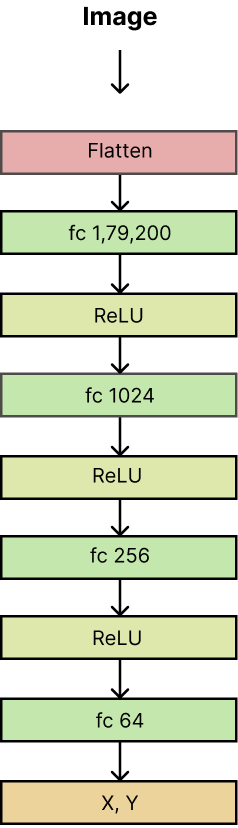
\includegraphics[width=0.2\columnwidth]{results/model.png}\\
 \captionof{figure}{architecture diagram}\label{pinki}
}

\subsection{Dataset} 

\par \noindent
A digital twin of the robot was created and simulated in a replica of the Robocon 2025 arena 
using the Gazebo \cite{gazebo} simulator with the help of ROS 2 \cite{macenski2022ros2}. 

\par \noindent
The robot was driven through the arena capturing images and corresponding $x$, $y$ coordinates. A 
TimeSynchronizer was used to synchronize the frame header and the position header. A total of
6283 images were captured and split into training  and test datasets with a 0.9 to 0.1 ratio.
Care was taken to include every part of the arena for an unbiased dataset. 

% maybe could get a better photo?
{ \centering
 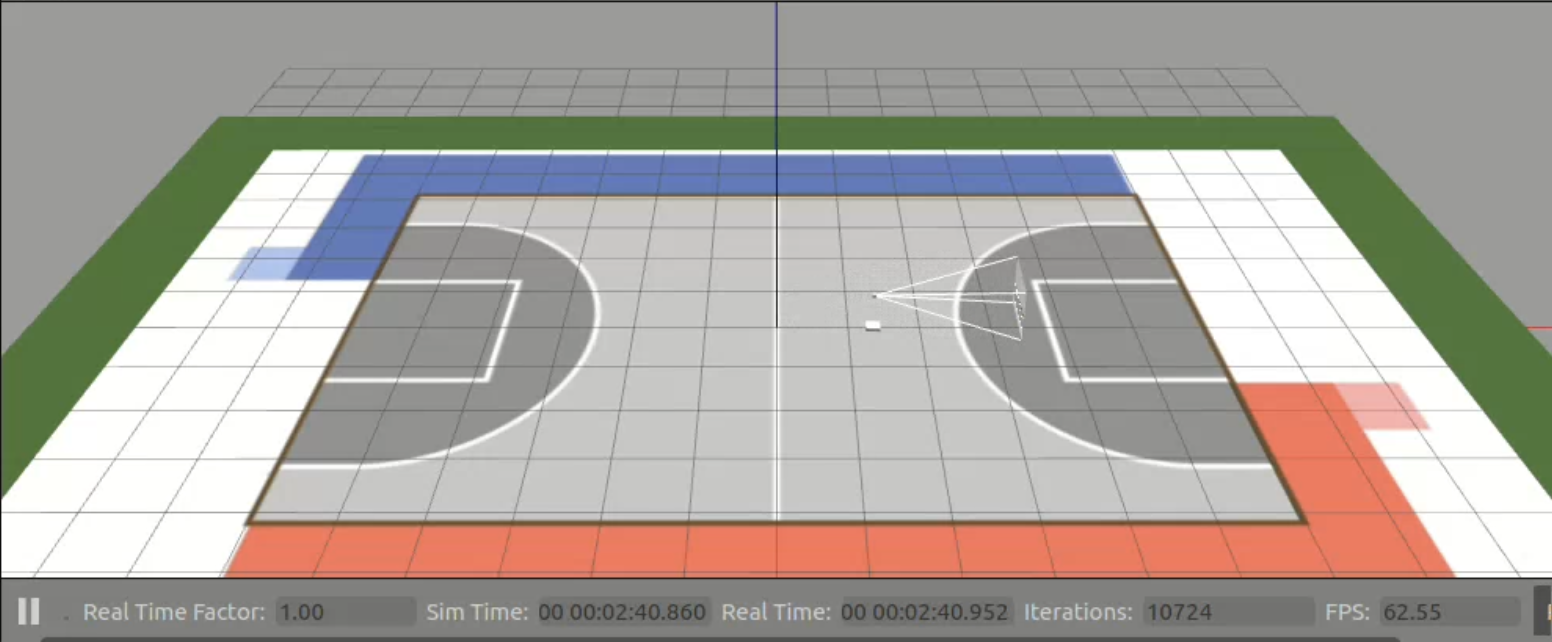
\includegraphics[scale=0.3]{results/gazebo.png}\\
 \captionof{figure}{gazebo simulation}\label{pinki}
}

\subsection{Training}
\par \noindent
The model was trained for 15 epochs using an Adam optimizer \cite{kingma2014adam} with an initial learning rate of $10^{-4}$
and a Mean Squared Error (MSE) cost function in batches of size 8. 

\section{Results}
% add repo link as well
\par \noindent
Figure IV depicts the loss at each epoch throughout the training process.
8 independent images at different points of the court were again captured 
from the simulation and fed into the model, Figure V shows the plot between
the ground truth and the prediction made with an average loss of 0.06 meters.

\par \noindent 
The code for the paper can be found in the following repository
\href{https://github.com/NarenTheNumpkin/Basketball-robot-localization}{https://github.com/NarenTheNumpkin/Basketball-robot-localization}

{ \centering
 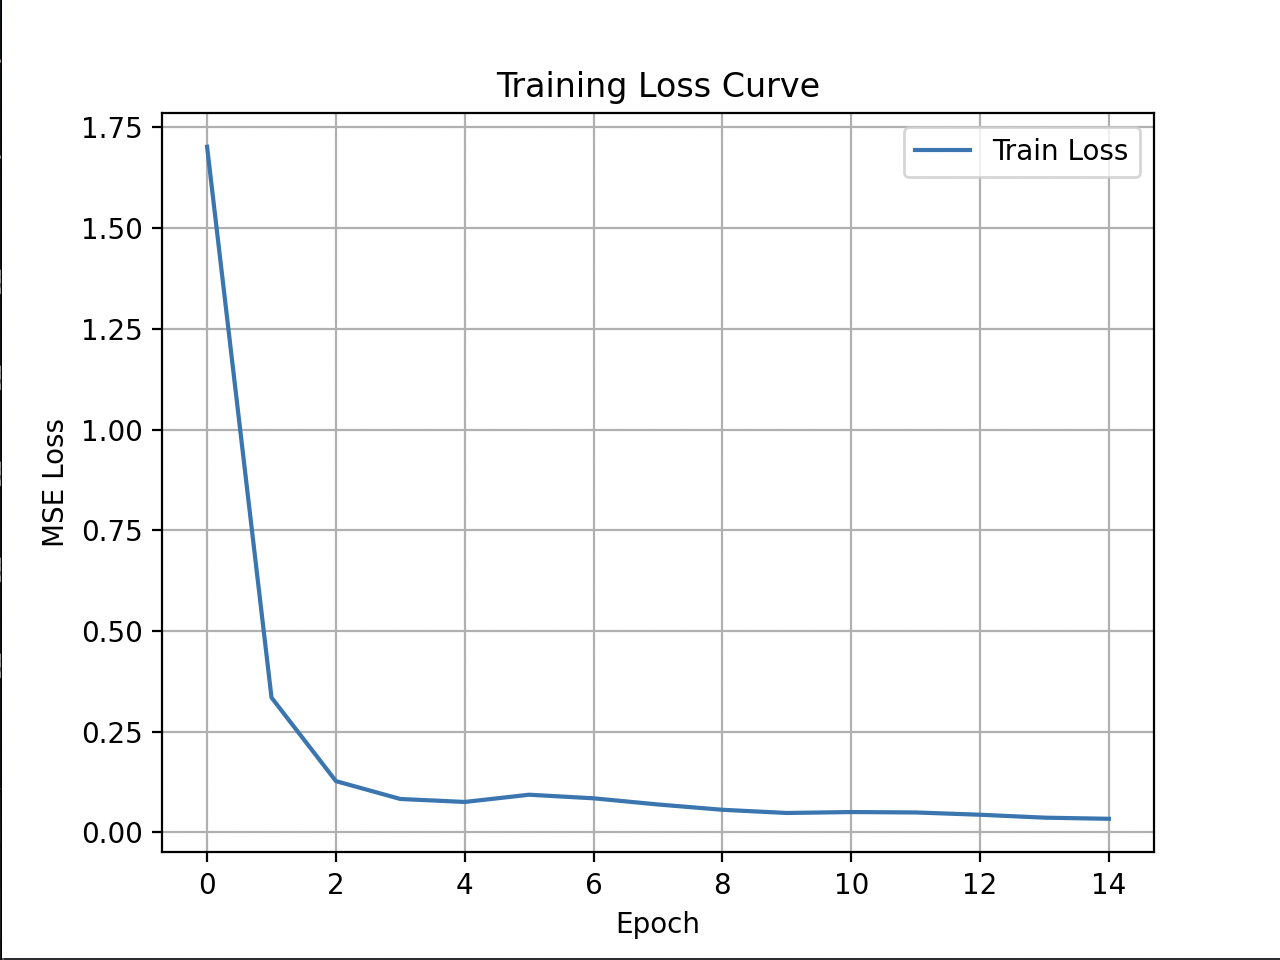
\includegraphics[scale=0.3]{results/loss-epochs.png}\\
 \captionof{figure}{loss curve}\label{pinki}
}

{ \centering
 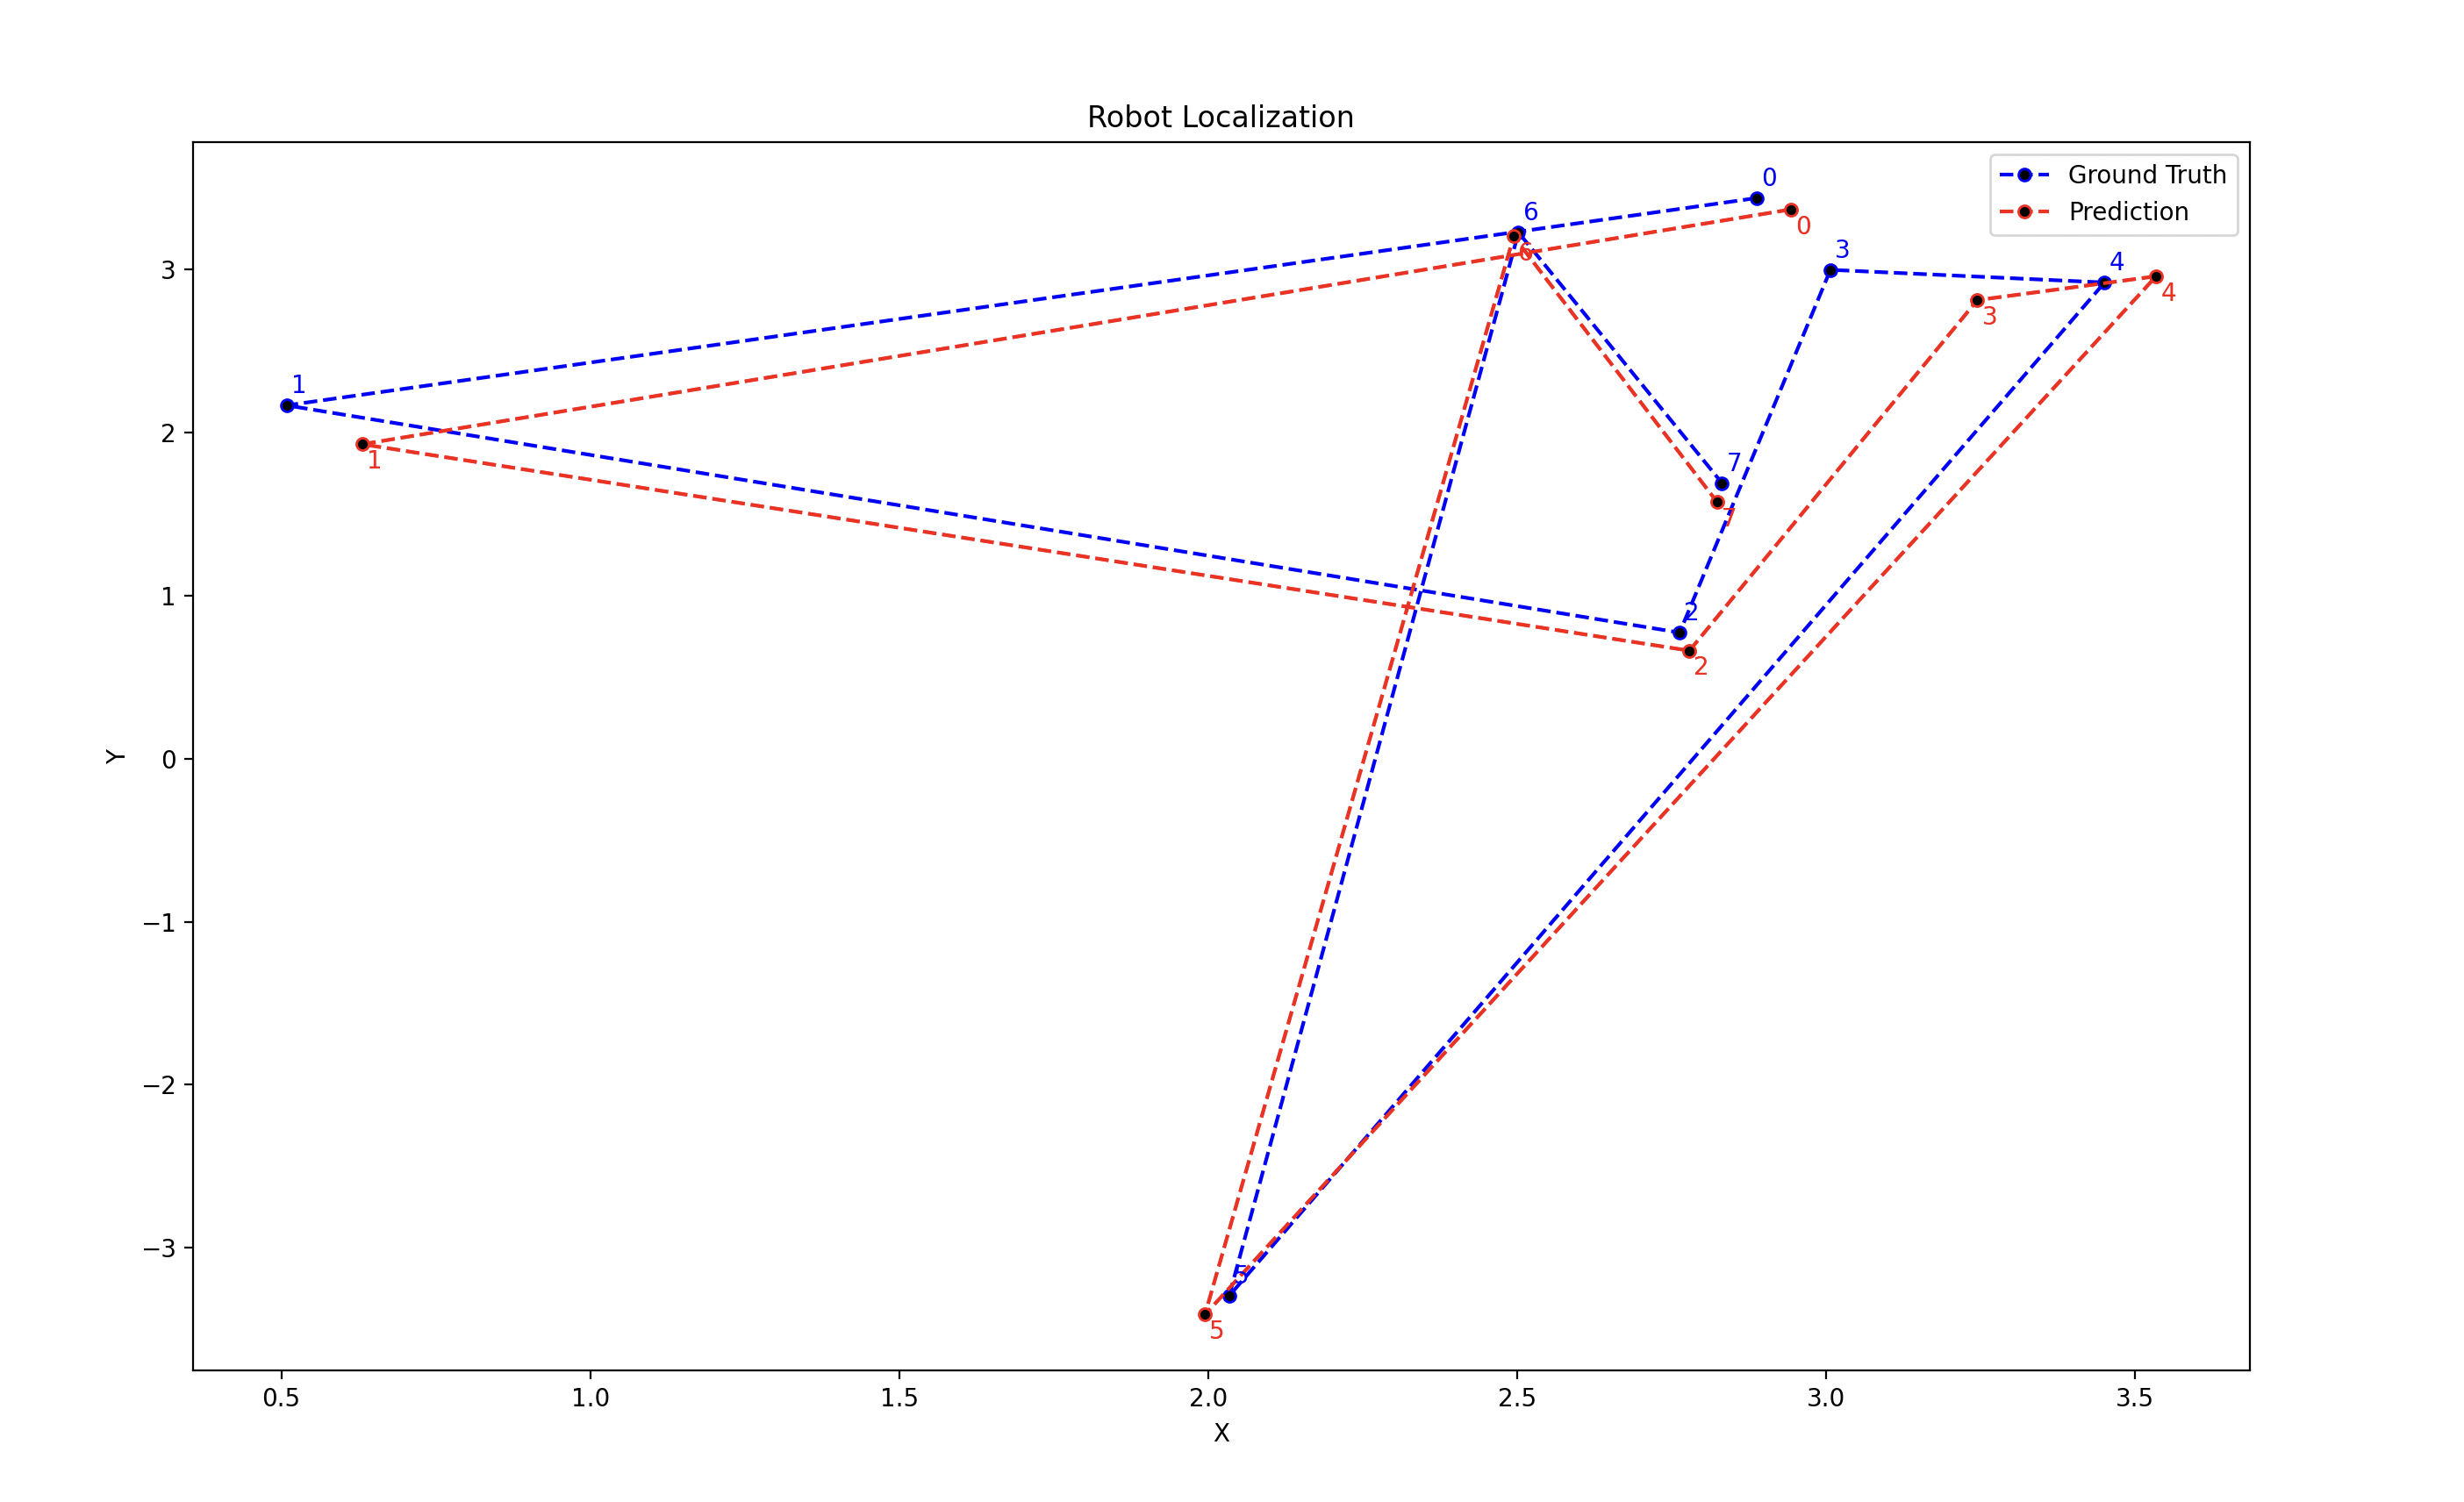
\includegraphics[scale=0.2]{results/comparison.png}\\
 \captionof{figure}{truth vs prediction}\label{pinki}
}

\section{Conclusion}  
\par \noindent
In this work, we presented a hybrid localization framework for autonomous basketball robots competing 
in the Robocon 2025 arena. Our approach relies solely on floor images processed through a lightweight
feedforward neural network. By preprocessing the images to highlight salient floor features and using a simple architecture, 
we achieved an average prediction error of approximately 0.06 meters, demonstrating the potential of 
learning-based localization methods. This result shows that even with minimal sensor inputs and modest 
model complexity, it is possible to achieve sufficiently accurate localization. Future improvements could 
focus on integrating other sensors such as IMU, wheel odometry, or LIDAR with the vision-based system 
through filtering techniques like Kalman or particle filters to achieve more robust and reliable 
localization. Additionally, exploring more neural network architectures may help to improve prediction 
accuracy. Finally, optimizing the model for deployment on embedded platforms with limited computational
resources through techniques such as pruning, quantization, or hardware acceleration could be worked upon.

\begin{thebibliography}{99}

\bibitem{gazebo}
N. Koenig and A. Howard, "Design and use paradigms for Gazebo, an open-source 
multi-robot simulator," 2004 IEEE/RSJ International Conference on Intelligent Robots 
and Systems (IROS) (IEEE Cat. No.04CH37566), Sendai, Japan, 2004, pp. 2149-2154 vol.3, 
doi: 10.1109/IROS.2004.1389727.
  
\bibitem{macenski2022ros2}
Steve Macenski, Tully Foote, Brian Gerkey, Chris Lalancette, and William Woodall. 
\textit{Robot Operating System 2: Design, architecture, and uses in the wild}. 
Science Robotics, vol. 7, no. 66, 2022. 

\bibitem{kingma2014adam}
Diederik P. Kingma and Jimmy Ba. 
\textit{Adam: A method for stochastic optimization}. 
arXiv preprint arXiv:1412.6980, 2014.

\end{thebibliography}

\end{multicols}

\end{document}
